\section{EXPERIMENTS}
In this section, I elaborate the details of the experiments and compare my model to several existing approaches in a real large dataset.
\subsection{Dataset}
The experiment is conducted in a real large dataset: MovieLens(100K). MovieLens\footnote{http://grouplens.org/datasets/movielens/} is a famous web-based research recommendation system, which is maintained by the Grouplens Research team at the University of Minnesota. And the MovieLens datasets are collected by the research team, one of which is the MovieLens(100K). The MovieLens(100K) contains 100,000 ratings(1-5 scales) rated by 943 users on 1682 movies, and each user at least rated 20 movies. The density of the user-item matrix is :
\begin{align*}
	\frac{100000}{943 \times 1682} = 6.30\%,
\end{align*}

The statistics of dataset MovieLens(100K) is summarized in table \ref{stats}. Besides, it also contains movie genre and titles. To increase the text information of very movie, a webpage crawler is employed to obtain the description of every movie from IMDB\footnote{http://www.imdb.com/}, which is a very famous movie website. For example, the description of the latest popular movie \textit{Forrest Gump}
is as follows:

\textit{Forrest Gump is a simple man with a low I.Q. but good intentions. He is running through childhood with his best and only friend Jenny. His 'mama' teaches him the ways of life and leaves him to choose his destiny. Forrest joins the army for service in Vietnam, finding new friends called Dan and Bubba, he wins medals, creates a famous shrimp fishing fleet, inspires people to jog, starts a ping-pong craze, create the smiley, write bumper stickers and songs, donating to people and meeting the president several times. However, this is all irrelevant to Forrest who can only think of his childhood sweetheart Jenny Curran. Who has messed up her life. Although in the end all he wants to prove is that anyone can love anyone.}

Then LDA model is executed in the text of information including title, genre, and the description, after which we can cluster the movies into different clusters, i.e. domains.
\begin{table}[]
	\centering
	\caption{Statistics of Dataset MovieLens(100K)}
	\label{stats}
	\begin{tabular}{|l|l|l|l|l|}
		\hline
		Statistics  & User  & Item   \\ \hline
		Min. Num. of Ratings  &20  &1   \\ \hline
		Max. Num. of Ratings  &737  &583  \\ \hline
		Avg. Num. of Ratings  &106.04  &59.45  \\ \hline
	\end{tabular}
\end{table}

\subsection{Performance Measures}
I perform 5-fold cross validation in the experiments. In each fold, 80\% of the data are used as training data and the rest as test data. I choose two evaluation metrics: Mean Absolute Error (MAE) and Root Mean Square Error (RMSE), which are the most popular accuracy measures in the literature of recommendation systems.
MAE is defined as
\begin{equation}
MAE = \frac{\sum_{(u,v) \in \mathcal{R}_{test}}{|R_{u,v} - \hat{R}_{u,v}|}}{|\mathcal{R}_{test}|},
\end{equation} 
where $\mathcal{R}_{test}$ is the set of all user\-item pairs (u,v) in the test set. And RMSE is defined as
\begin{equation}
RMSE = \sqrt{\frac{\sum_{(u,v) \in \mathcal{R}_{test}}{(R_{u,v} - \hat{R}_{u,v})^2}}{|\mathcal{R}_{test}|}}.
\end{equation}
\subsection{Evaluation}
In order to demonstrate the effectiveness of the proposed IDSR model, I compare the recommendation result with several baselines in the following:
\begin{itemize}
	\item \textbf{GlobalAVG}: it uses the average of the ratings of all the observed items as predictions.
	\item \textbf{UserAVG}: it uses the average of ratings given by the user as his/her predictions.
	\item \textbf{ItemAVG}: it uses the average of ratings received by the target item as its predictions.
	%\item \textbf{UserKNN}: In this method, a set of similar users are firstly found, the predicted rating of this user on one item is calculated as weighted average of the similar users' ratings of the item.
	%\item \textbf{ItemKNN}: The method is very similar to the \textbf{UserKNN}, just take the weighted average of the similar items' rating as the predicted rating of the item.
	\item \textbf{NMF} this method is originally proposed in \cite{lee1999learning} for image analysis. However, it is widely used in collaborative filtering recently. It only uses user-item matrix for recommendation.
	\item \textbf{PMF}: This is the basic matrix factorization approach propose in \cite{mnih2007probabilistic} , which does not take into account the social network.
\end{itemize}

The reason why I don't choose recent work which integrate the social factor into matrix factorization framework \cite{jamali2010matrix}\cite{ma2008sorec}\cite{ma2009learningTrust}\cite{yang2012circle}\cite{yang2013social} is that they all require explicit connections between users like following in twitter or trust in Epinion\footnote{https://snap.stanford.edu/data/soc-Epinions1.html}

\subsection{Comparisons}
The MAE and RMSE results are showed in table \ref{rmse&mael}
\begin{table}[]
	\centering
	\caption{Comparisons}
	\label{rmse&mael}
	\begin{tabular}{|c|c|c|c|c|}
		\hline
		\multicolumn{1}{|l|}{} & \multicolumn{2}{c|}{d=5} & \multicolumn{2}{c|}{d=10} \\ \hline
		\multicolumn{1}{|l|}{} & MAE(improve) & RMSE(improve) & MAE(improve) & RMSE(improve) \\ \hline
		\textbf{GlobalAVG} & 0.945(23.28\%) & 1.126(18.38\%) & 0.945(24.76\%) & 1.126(18.92\%) \\ \hline
		\textbf{UserAVG} & \textbf{0.835(13.17\%)} & 1.042(11.80\%) & 0.835(14.85\%) & 1.042(12.38\%) \\ \hline
		\textbf{ItemAVG} & 0.817(11.26\%) & 1.025(10.34\%) & 0.817(12.97\%) & 1.025(10.93\%) \\ \hline
		\textbf{NMF} & 0.727(0.28\%) & 0.92(0.11\%) & 0.736(3.40\%) & 0.945(3.39\%) \\ \hline
		\textbf{PMF} & 0.747(2.95\%) & 0.926(0.76\%) & 0.715(0.56\%) & 0.919(0.65\%) \\ \hline
		\textbf{IDSR} & \textbf{0.725} & \textbf{0.919} & \textbf{0.711} & \textbf{0.913} \\ \hline
	\end{tabular}
\end{table}

For \textbf{GlobalAVG,UserAVG, ItemAVG}, they have no extra parameters, including the dimensionality, thus we just keep the rmse\&mae the same in different dimensionality for the convenience of comparison. For \textbf{PMF} and my \textbf{IDSR}, the $\lambda_1$ and $\lambda_2$ are set to 0.001 as previous work did. And the regularization parameter $\beta$ is very important, which control how much my method should incorporate the information of the trust network. The larger value of $\beta$ is chosen, the more influence will the trust network will exert on the recommendation process. The detail of this change is given in the following. And $\beta$ is set to 0.01 here for its good performance.

Another parameter is the number of topic number in the clustering process. For the result reported, we set it to 30 for its good performance too.

From the result in the table \ref{rmse&mael}, we can see that my method outperform other baseline models consistently, demonstrating the effectiveness of integrating the implicit trust information between users.

\subsection{Impact of the number K of domains and regularization $\beta$}
As mentioned in the above section, the parameter $K$ and $\beta$ are very important. $K$ controls how many topics (i.e.domains) we choose when clustering the items, while $\beta$ decide how much influence the trust will exert on recommendation process. In this section, I analyze the changes of $K$ and $\beta$ can affect the final recommendation accuracy.

\begin{figure}[h]
	\caption{Impact of $\beta$}
	\label{fig:beta}
	%\centering
	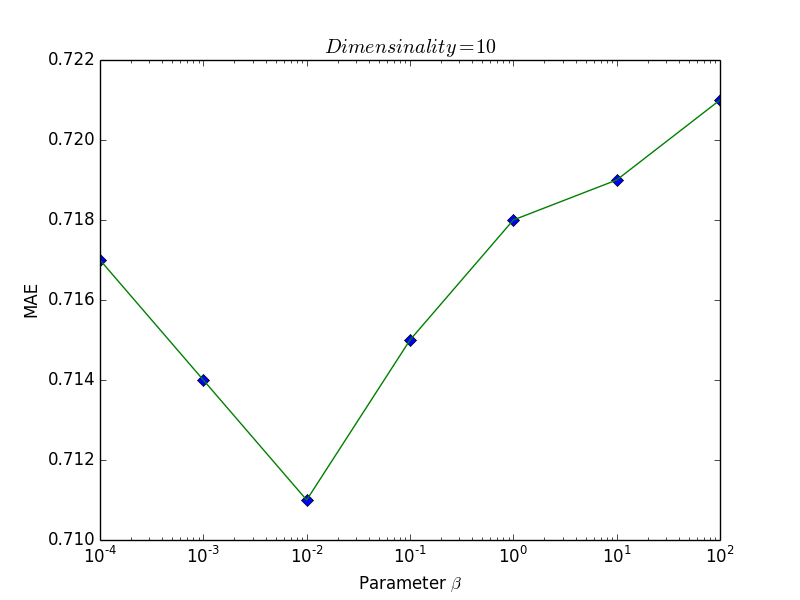
\includegraphics[width=8cm]{beta_mae}
	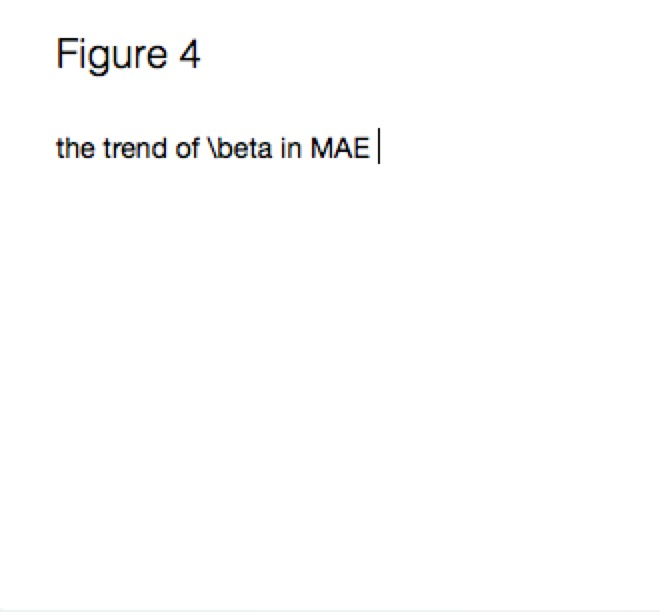
\includegraphics[width=8cm]{beta_rmse}
\end{figure}

Figure \ref{fig:beta} shows the impacts of $\beta$ on MAE and RMSE in the \textbf{IDSR} model. We observe that no matter how much is $\beta$, MAE and RMSE decreases comparing with $\beta = 0$, which demonstrate the effectiveness of integrating the trust information. Besides, there is a threshold like 0.01 for $\beta$, the MAE and RMSE values increases with further increase of the value $\beta$. This confirm with the intuition that purely using the rating matrix or purely using the trust network information for recommendation cannot generate better performance than appropriately integrating these two sources together.

The analysis of $K$ is very similar to $\beta$, which shows that $K$ cannot be too large or too small.(See Figure \ref{fig:k})
\begin{figure}[h]
	\caption{Impact of $K$}
	\label{fig:k}
	%\centering
	\includegraphics[width=8cm]{K_mae}
	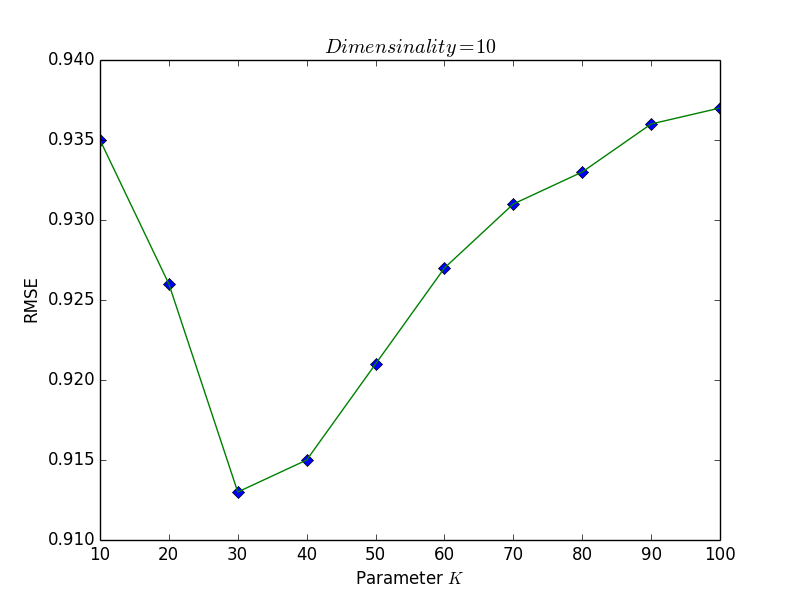
\includegraphics[width=8cm]{K_rmse}
\end{figure}

